\providecommand{\setflag}{\newif \ifwhole \wholefalse}
\setflag
\ifwhole\else

% Typography and geometry ----------------------------------------------------
\documentclass[letterpaper]{scrbook}
\usepackage[inner=3cm,top=2.5cm,outer=3.5cm]{geometry}

\renewcommand\familydefault{bch}
\usepackage[utf8]{inputenc}
\usepackage{microtype}
\usepackage[small]{caption}
\usepackage[small]{titlesec}
\raggedbottom

% Graphics -------------------------------------------------------------------
\usepackage[pdftex]{graphicx}
\graphicspath{{_include/}}
\DeclareGraphicsExtensions{.png,.pdf}

% Code formatting ------------------------------------------------------------
\usepackage{fancyvrb}
\usepackage{courier}
\usepackage{listings}
\usepackage{color}
\usepackage{alltt}


\definecolor{comment}{rgb}{0.60, 0.60, 0.53}
\definecolor{background}{rgb}{0.97, 0.97, 1.00}
\definecolor{string}{rgb}{0.863, 0.066, 0.266}
\definecolor{number}{rgb}{0.0, 0.6, 0.6}
\definecolor{variable}{rgb}{0.00, 0.52, 0.70}
\lstset{
  basicstyle=\ttfamily,
  keywordstyle=\bfseries, 
  identifierstyle=,  
  commentstyle=\color{comment} \emph,
  stringstyle=\color{string},
  showstringspaces=false,
  columns = fullflexible,
  backgroundcolor=\color{background},
  mathescape = true,
  escapeinside=&&,
  fancyvrb
}
\newcommand{\code}[1]{\lstinline!#1!}
\newcommand{\f}[1]{\lstinline!#1()!}



% Links ----------------------------------------------------------------------

\usepackage{hyperref}
\definecolor{slateblue}{rgb}{0.07,0.07,0.488}
\hypersetup{colorlinks=true,linkcolor=slateblue,anchorcolor=slateblue,citecolor=slateblue,filecolor=slateblue,urlcolor=slateblue,bookmarksnumbered=true,pdfview=FitB}
\usepackage{url}

% Tables ---------------------------------------------------------------------
\usepackage{longtable}
\usepackage{booktabs}

% Miscellaneous --------------------------------------------------------------
\usepackage{pdfsync}
\usepackage{appendix}

\usepackage[round,sort&compress,sectionbib]{natbib}
\bibliographystyle{plainnat}


\title{ggplot2}
\author{Hadley Wickham}

\begin{document}
\fi


\chapter{Aesthetic specifications}
\label{cha:specifications}

This appendix summarises the various formats that \code{grid} drawing functions take.  Most of this information is available scattered throughout the R documentation.  This appendix brings it all together in one place.

\section{Colour}
\label{sec:colour_spec}

Colours can be specified with:

\begin{itemize}
  \item A {\bf name}, e.g.\ \code{"red"}. The colours are displayed in Figure~\ref{fig:colours}, and can be listed in more detail with \f{colours}. The Stower's institute provides a nice printable pdf that lists all colours:  \url{http://research.stowers-institute.org/efg/R/Color/Chart/}.
    
  \item An {\bf rgb specification}, with a string of the form \code{"#RRGGBB"} where each of the pairs \code{RR}, \code{GG}, \code{BB} consist of two hexadecimal digits giving a value in the range \code{00} to \code{FF}.  Partially transparent can be made with \f{alpha}, e.g.\ \code{alpha("red", 0.5)}

  \item An {\bf NA}, for a completely transparent colour.  
\end{itemize}

The functions \f{rgb}, \f{hsv}, \f{hcl} can be used to create colours specified in different colour spaces.

% The \f{diverge_hcl}, \f{sequential_hcl}, \f{rainbow_hcl}, and \f{heat_hcl} functions from the \code{vcd} package provide other ways of generate colours palettes based on perceptually sound principles.

\section{Line type}
\label{sec:line_type_spec}

Line types can be specified with:

\begin{itemize}
  \item A {\bf integer} or {\bf name}: 0=blank, 1=solid, 2=dashed, 3=dotted, 4=dotdash, 5=longdash, 6=twodash), illustrated in Figure~\ref{fig:linetype}

  \item The lengths of on/off stretches of line. This is done with a string of an even number (up to eight) of hexadecimal digits which give the lengths in consecutive positions in the string. For example, the string \code{"33"} specifies three units on followed by three off and \code{"3313"} specifies three units on followed by three off followed by one on and finally three off. 
  
  The five standard dash-dot line types described above correspond to 44, 13, 134, 73, and 2262.
\end{itemize} 

Note that \code{NA} is not a valid value for \code{lty}.

\section{Shape}
\label{sec:shape_spec}

Shapes take four types of values:

\begin{itemize}
  \item An {\bf integer} in $[0, 25]$, illustrated in Figure~\ref{fig:shape}.

  \item A {\bf single character}, to use that character as a plotting symbol.   

  \item A \code{.} to draw the smallest rectangle that is visible (i.e. about one pixel).
  
  \item An {\bf NA}, to draw nothing.
\end{itemize}

While all symbols have a foreground colour, symbols 19--25 also take a background colour (fill). 

\section{Size}
\label{sec:size}

Throughout \ggplot, for text height, point size and line width, size is specified in millimetres.

\section{Justification}
\label{sec:justification_spec}

Justification of a string (or legend) defines the location within the string that is placed at the given position.  There are two values for horizontal and vertical justification.  The values can be:

\begin{itemize}
  \item A {\bf string}: \code{"left"}, \code{"right"}, \code{"centre"}, \code{"center"}, \code{"bottom"}, and \code{"top"}.
  
  \item A {\bf number} between 0 and 1, giving the position within the string (from bottom-left corner).  These values are demonstrated in Figure~\ref{fig:justification}.
\end{itemize}

\begin{figure}[htbp]
  \centering
  \subfigure[All named colours in Luv space]{
    \label{fig:colours}
    \includegraphics[width=0.45\textwidth]{scale-identity}
  }
  \subfigure[Built-in line types]{
    \label{fig:linetype}
    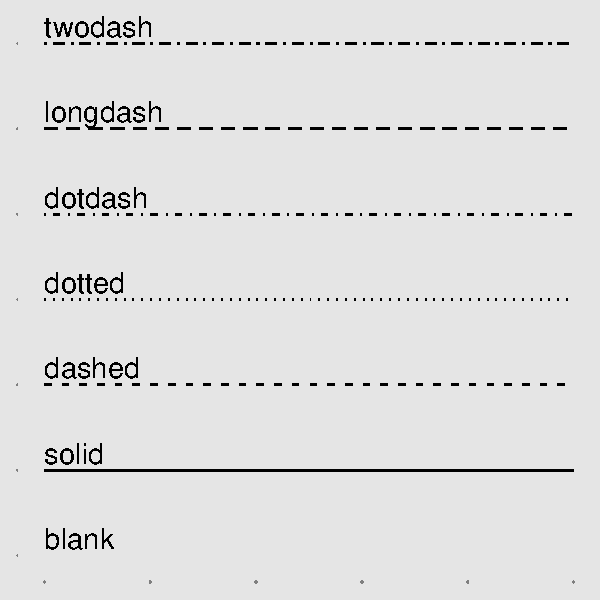
\includegraphics[width=0.45\textwidth]{spec-linetype}
  }
  \subfigure[R plotting symbols.  Colour is black, and fill is blue.  Symbol 25 (not shown) is symbol 24 rotated 180 degrees.]{
    \label{fig:shape}
    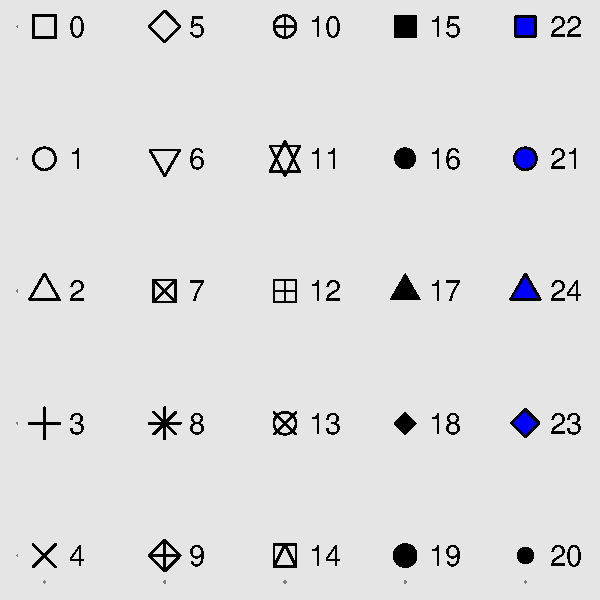
\includegraphics[width=0.45\textwidth]{spec-shape}  
  }
  \subfigure[Horizontal and vertical justification settings.]{
    \label{fig:justification}
    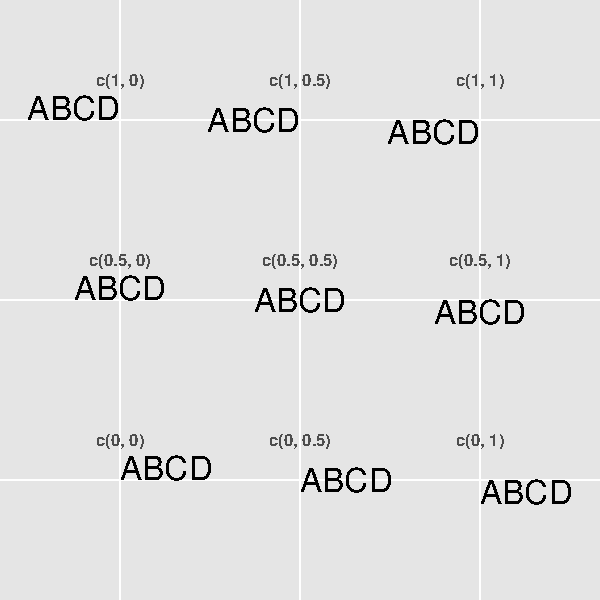
\includegraphics[width=0.45\textwidth]{spec-justification}
  }
  \caption{Examples illustrating different aesthetic settings.}
\end{figure}

\section{Fonts}
\label{sec:fonts}

postscriptFonts, pdfFonts, quartzFonts

Find R news article

\begin{itemize}
  \item \code{face}
  \item \code{family}
  \item \code{lineheight}
  \item \code{fontsize}
\end{itemize}


% section fonts (end)

\ifwhole
\else
  \nobibliography{/Users/hadley/documents/phd/references}
  \end{document}
\fi